\section{Resultate}\label{resultate}
Wie im Kapitel \ref{konzept} wird erwähnt, dass der Ist-Zustand die Feldlinien im FITS-Dateiformat abspeichert. Es wurde geprüft, wie viel Speicher das Format nach der Entropie-Kodierung beansprucht. Für den Test wurde die Komprimierung \ref{resultate:loesung0} werwendet. Zum Vergleich wurden die Daten im FITS-Dateiformat und als Binärdatei abgelegt.
\begin{table}[!htbp]
\center
\begin{tabular}{c|c}
	 pro Feldlinie (FITS) & Bytes pro Feldlinie (Binär)\\\hline
	$74.2$ Bytes & $73.6$ Bytes\\
\end{tabular}
\caption{Einfluss des FITS Formates auf den Speicherverbrauch}
\label{resultate:fits_table}
\end{table}
Die Resultate \ref{resultate:fits_table} zeigen keinen signifikanten Unterschied des Speicherverbrauchs. Pro Feldlinie liegt der Unterschied bei $0.6$ Bytes. Hochgerechnet auf $1200$ Feldlinien sind es 0.7 KiBytes, welches das Fits-Format für sich beansprucht. Fits erlaubt es, den Datenreihen einen Namen so wie eine kurze Beschreibung anzuhänken. Diese Strings sind Optional und können auch weggelassen werden.\\
Der wesentliche Vorteil von FITS ist, dass es bereits Plattformunabhängig ist. Probleme wie Endianness \cite{wiki:endianess} werden vom Format gelöst. Aus diesen Gründen wurde entschieden das Format beizubehalten.

\subsection{Lösung 0, Angle-Subsampling} \label{resultate:loesung0}
Das Angle-Subsampling führt der JHelioviewer selbst durch. Für die Lösung 0 soll nun das Subsampling vor der Dateiübertragung vorgenommen werden. Dazu werden die Punkte in das kartesische Koordinatensystem umgerechnet, das Angle-Subsampling durchgeführt und anschliessend wird in das sphärische System rücktransformiert. Die resultierende FITS-Datei wird mittels Rar kodiert.
\begin{figure}[!htbp]
	\center
	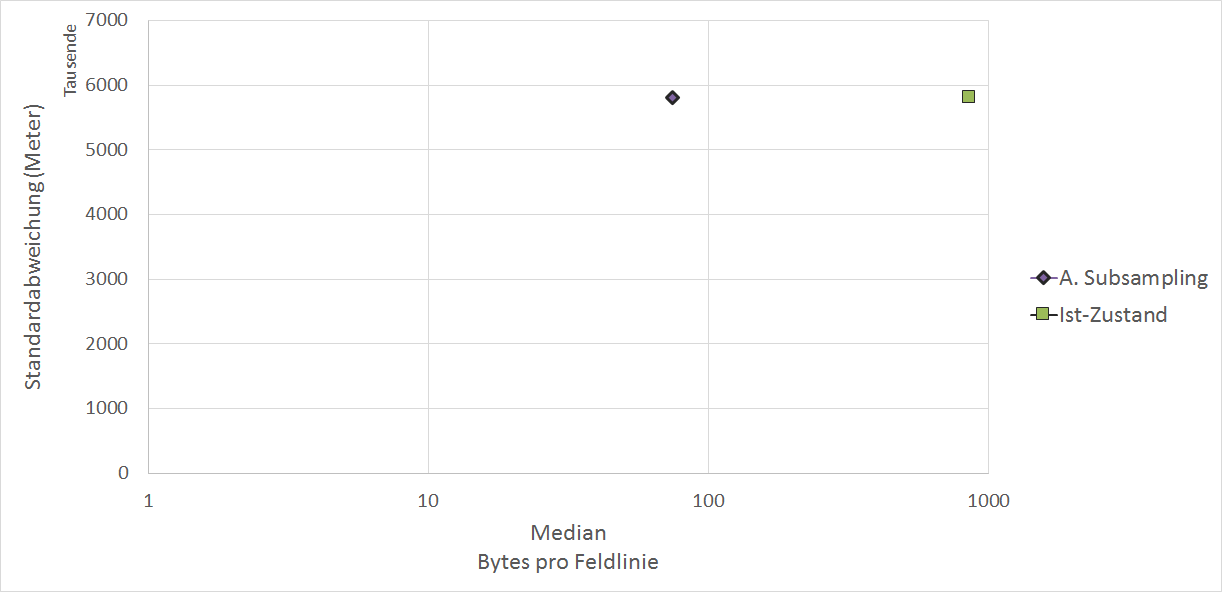
\includegraphics[width=0.8\textwidth,height=6cm,keepaspectratio]{./pictures/resultate/loesung0/loesung0_0.png}
	\caption{Vergleich der Lösung 0 zum Ist-Zustand.}
	\label{resultate:loesung0:loesung0_0}
\end{figure}
Wie im Diagramm \ref{resultate:loesung0:loesung0_0} erkennbar ist, verbraucht die Lösung 0 um grössenordnungen weniger Speicher. Zu einem wird durch das Angle-Subsampling weniger Daten gespeichert,etwa nur ein Viertel der ursprünglichen Punkte. Zum anderen erbringt Rar die bessere Kompression. Die Komplexität der Kompression und Dekompression bleibt in der Grössenordnung $O(n)$ ($n$ ist die Anzahl Punkte). Da bei der Dekompression $n$ etwa vier Mal weniger Punkte bearbeiten muss, ist die Dekompression sogar schneller als die Ist-Lösung.
\begin{figure}[!htbp]
	\center
	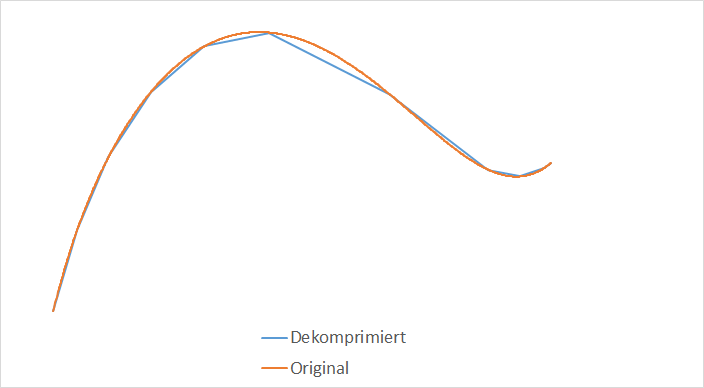
\includegraphics[width=0.8\textwidth,height=6cm,keepaspectratio]{./pictures/resultate/loesung0/loesung0_artefakte.png}
	\caption{Artefakte der Lösung 0}
	\label{resultate:loesung0:artefakte}
\end{figure}
Die Abbildung \ref{resultate:loesung0:artefakte} zeigt die Artefakte, die bei der Komprimierung der Lösung 0 entstehen. Aus dem JHelioviewer sind diese Artefakte kaum sichtbar.

\subsection{Lösung 1, Diskrete Kosinus Transformation}
Das Ziel ist eine bessere Kompression zu erreichen, indem die Feldlinien mit Kosinusfunktionen approximiert werden. 
Die DCT-Implementierung für die Tests weist eine Komplexität von $O(n^2)$. Bei etwa $600$ Punke pro Linie ist das zu erheblichen Rechenaufwand. Deshalb wird vor der DCT deshalb ein Subsampling durch. Falls die Laufzeit der Dekompression verbessert werden soll, kann die Fast-Cosine-Transformation umgesetzt werden. Diese hat eine Komplexität von $O(n logn)$. Falls das nicht ausreicht, können die Linien in Blöcken mit einer bestimmten Anzahl von Punkten unterteilt werden. Das senkt die Komplexität auf $O(n)$. Die Unterteilung könnte negative Effekte auf die Kompression haben.\\
[\baselineskip]
In den Tests wurde eine lineare Quantisierung verwendet. Jeder DCT Koeffizient wird durch einen Faktor geteilt, der sich stetig ehöht. Zum Beispiel wird der erste Koeffizient durch zwei geteilt, der zweite durch Vier, der Dritte durch Sechse etc.  Die Kompressionsrate kann durch einen höheren oder tieferen Faktor gesteuert werden. Diese Quantifizierung ist nicht das Optimum. Eine bessere Quantifizierung wird für die beste Lösung ausgearbeitet.

\subsubsection{DCT}\label{resultate:dct}
Nach dem Subsampling wird auf den Punkten (im kartesischen Koordinatensystem) die Diskrete Kosinus Transformation ausgeführt. Es ist auch möglich die Punkte im sphärischen Koordinatensystem in den Frequenzraum zu überführen. Der $\phi$-Kanal ist jedoch schwierig durch tiefe Kosinus schwingungen darzustellen: Wie im Abschnitt \ref{konzept:ist-komprimierung} besprochen, beinhaltet der Kanal Sprünge bei der Passierung des Nullpunktes. Das führt zu sehr hochfrequenten Schwingungsanteile in der DCT. Nach einer Quantisierung sind dabei Artefakte nicht vermeidbar. Im kartesischen System hingegen sind alle Kanäle stetig und haben somit wenige hochfrequente Anteile.\\
Die Anzahl Punkte pro Linie werden zuerst als 16 Bit Integer Array abgelegt, gefolgt von allen DCT Koeffizienten des X Kanals, danach des Y und zum Schluss des Z Kanals mit 32 Bit Genauigkeit.\\
\begin{figure}[!htbp]
	\center
	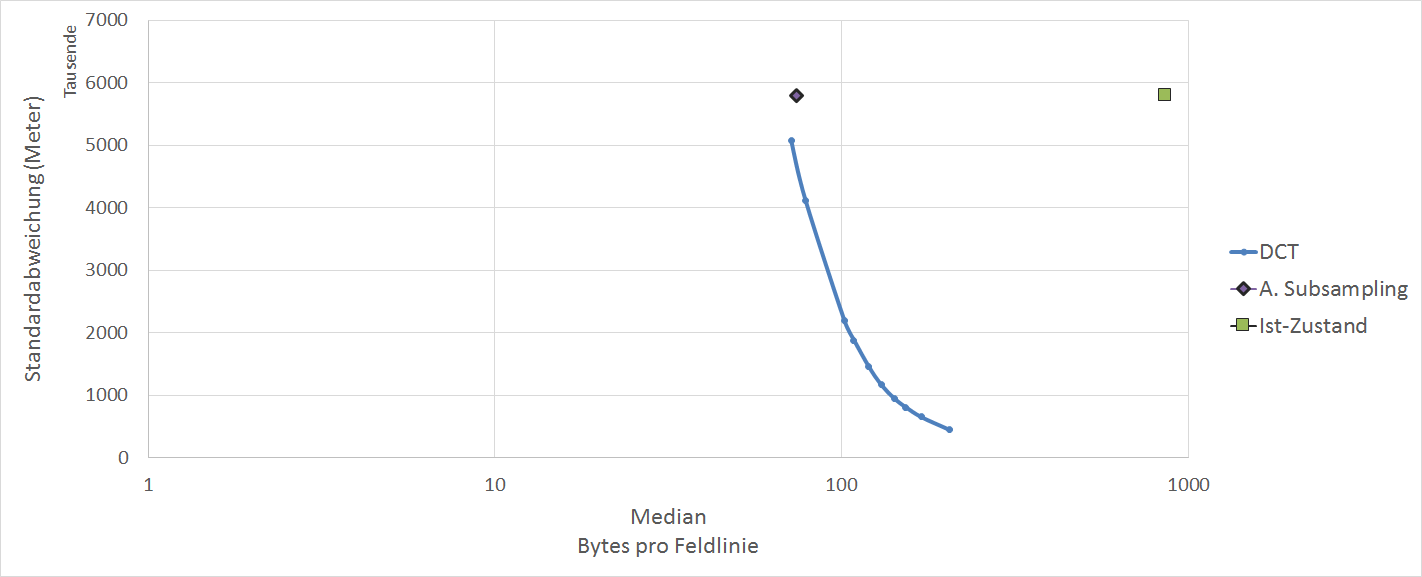
\includegraphics[width=0.8\textwidth,height=6cm,keepaspectratio]{./pictures/resultate/loesung1/loesung1-0/loesung1_0.png}
	\caption{Vergleich der DCT Kompression mit der Lösung0}
	\label{resultate:loesung1:dct:resultate}
\end{figure}
Die Abbildung \ref{resultate:loesung1:dct:resultate} zeigt den Vergleich der DCT Kompression mit der Lösung 0. Es ist deutlich zu erkennen, dass die Standardabweichung schnell steigt bei leicht sinkender Grösse. Der Maximale Fehler steigt ebenfalls schnell und erreicht beim letzten Test eine höhe von $140'686'000$ Meter. Zum Vergleich: Der maximale Fehler der Lösung 0 ist mehr als vier Mal kleiner und liegt bei $30'014'000$ Meter.\\
\begin{figure}[!htbp]
	\center
	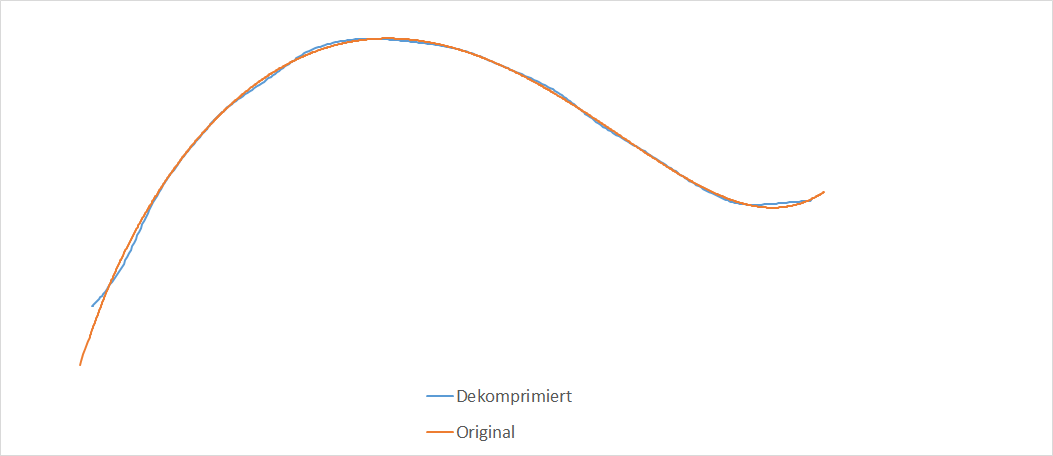
\includegraphics[width=0.8\textwidth,height=6cm,keepaspectratio]{./pictures/resultate/loesung1/loesung1-0/loesung1_0_artefakte.png}
	\caption{Artefakte der DCT Dekompression}
	\label{resultate:loesung1:dct:artefakte}
\end{figure}
Die Darstellung der Artefakte \ref{resultate:loesung1:dct:artefakte} zeigen das Problem: in den meisten Fällen kann die DCT die Feldlinie gut approximieren. Bei dieser Feldlinie wird der Anfang der Kurve nicht richtig dargestellt. Das ist ein typisches Problem der DCT: Die Transformation nimmt an, dass das Signal sich am Anfang und am Ende in umgekehrter Reihenfolge wiederholt \cite{wiki:dct}. Gerade beim Anfang bedeutet das ein Unterbruch, welche sich nur durch hochfrequente Anteile darstellen lässt.\\
Eine Möglichkeit ist die Feldlinie um Punkte zu erweitern, welche die Transformation vereinfachen. Wenn die Punkte geschickt gewählt werden, sollte eine Feldlinie nach der Transformation und Quantisierung ähnlich viele Bytes benötigen. Durch eine andere Darstellung könnten diese Probleme ebenfalls gelöst werden, weshalb zuerst weitere Transformationen analysiert werden.

\subsubsection{Feldlinien Ableiten mit DCT}\label{resultate:dct:ableitung_dct}
Bevor die Feldlinie Kosinus-Transformiert und Quantisiert wird, soll sie abgeleitet werden. Die Kosinustransformation wird auf den Steigungen ausgeführt. Damit die Operation umkehrbar ist, wird der Startpunkt der Feldlinie im kartesischen Koordinatensystem gespeichert. Mit der Ableitung sollen zu einem die Koeffizienten gedämpft werden, sodass sie sich mit weniger Genauigkeit quantisieren lassen. Zum Anderen soll das Randproblem dargestellt in \ref{resultate:loesung1:dct:artefakte} gelöst werden. Die Steigungen sind kleinere Zahlen, was nicht so einen starken Wechsel verursachen sollte. Der Nachteil ist, dass Ungenauigkeiten sich durch die Kurve durchziehen und summieren. Anfangs stimmen komprimierte und Originalkurve sehr genau überein. Aber gegen Ende können sie immer mehr abweichen.\\
Die DCT Koeffizienten und die X,Y und Z Kanäle der Startpunkte weren mit 16 Bit quantisierten getrennt abgelegt. Die DCT, die Quantisierung sowie die Entropie Kodierung ist die Selbe wie bei \ref{resultate:dct}.
\begin{figure}[!htbp]
	\center
	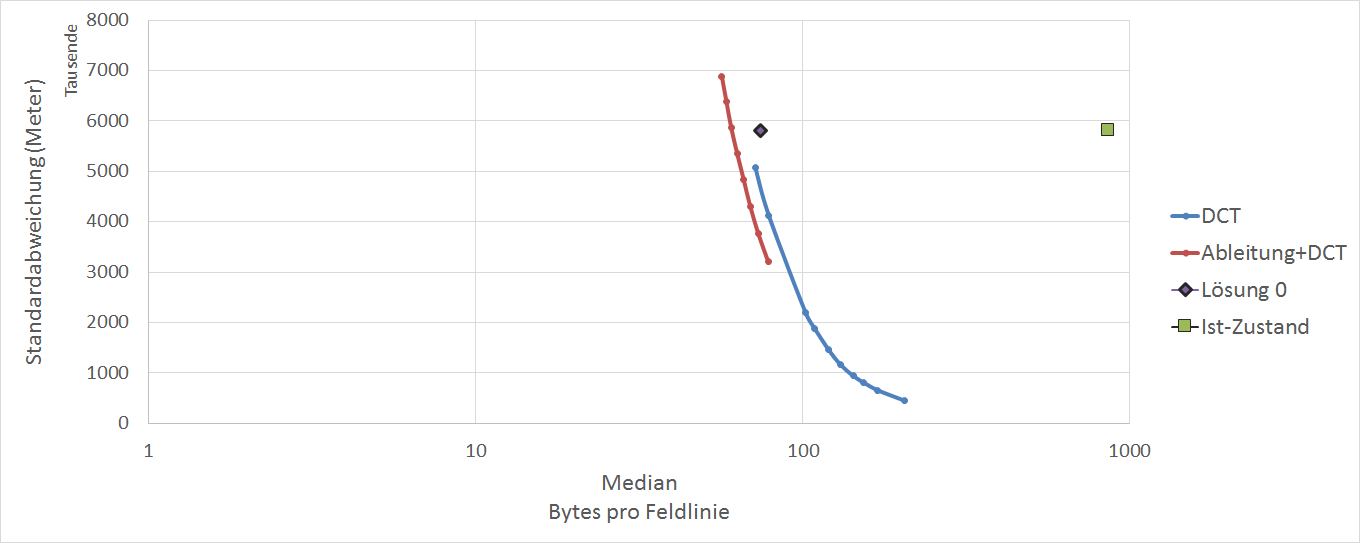
\includegraphics[width=0.8\textwidth,height=6cm,keepaspectratio]{./pictures/resultate/loesung1/loesung1-1/loesung1_1.png}
	\caption{Vergleich der DCT Kompression der Ableitung mit der DCT Kompression}
	\label{resultate:loesung1:dct:artefakte}
\end{figure}
Die abgeleiteten Feldlinien können sehr gut quantisiert werden. Im Vergleich zur Lösung 0 braucht diese Variante etwa 15 Byte weniger um eine Feldlinie darzustellen. Durchschnittlich ist jetzt eine PFSS Simulation auf 72 KiByte komprimiert.\\
Die Feldlinien liegen meist auf einer Ebene im dreidimensionalen Raum. Wenn die X,Y und Z Kanäle Kosinus-Transformiert werden, ist die Information etwa gleichmässig auf den Kanälen verteilt. Eine Linie könnte sich durch weniger Kosinus-Funktionen approximieren lassen, wenn die Linie zuerst in ein lokales Koordinatensystem transformiert wird. Die Koordinatenachsen können für jede Linie so gelegt werden, dass der X und Y Kanal den Grossteil der Informationen beinhalten. Der Z Kanal könnte für viele Feldlinien Null sein. Es wird vermutet, dass mit einem lokalen Koordinatensystem X und Y Kanäle etwa gleich viele Kosinus-Funktionen brauchen, aber der Z Kanal so gut wie keine. 

\subsubsection{Feldlinien Ableiten mit PCA und DCT}
Mit einer vorhergehenden Principal Component Analysis (PCA) \cite{abdi2010principal} werden die Feldlinien vom Sonnen-Koordinatensystem in ihr lokales System transformiert. 
PCA ist ein Verfahren aus der Statistik, welches Daten in ein neues koordinatensystem Transformiert. Dabei werden die Achsen so gelegt, dass die Daten entlang der ersten Achse die grösste Varianz aufweisen. Entlang der zweiten Achse, welche orthogonal zur ersten liegt, die zweithöchste Varianz etc. Wenn das Vefahren auf die Feldlinien angewandt wird, werden die Feldlinien in ein lokales System transformiert indem der Z-Kanal 0 ist, wenn die Feldlinie in einer Ebene liegt. Der Nachteil ist, dass für die Rücktransformation pro Feldlinie die Koordinatenachsen und die Koordinatenverschiebung abgespeichert werden. Für Achsen werden 16 Bit Genauigkeit und für die Verschiebung 32 Bit verwendet.
\begin{figure}[!htbp]
	\center
	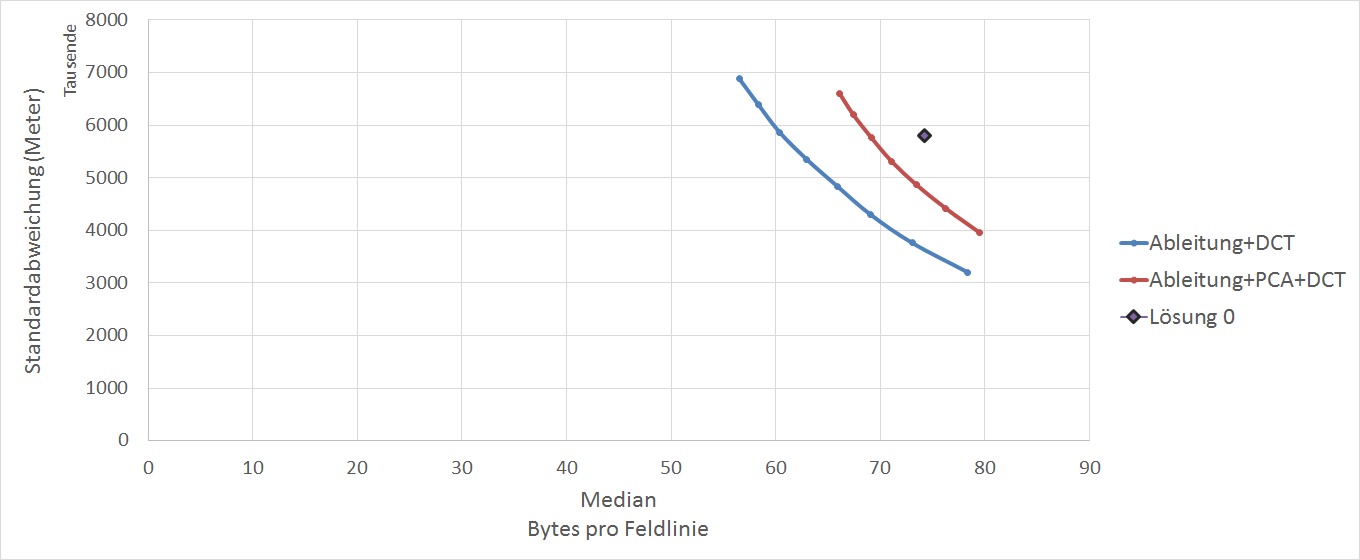
\includegraphics[width=0.8\textwidth,height=6cm,keepaspectratio]{./pictures/resultate/loesung1/loesung1-4/loesung1_4.png}
	\caption{Vergleich der PCA DCT Kompression der Ableitung mit der DCT Kompression der Ableitung}
	\label{resultate:loesung1:dct:pca}
\end{figure}
Der Vergleich \ref{resultate:loesung1:dct:pca} zeigt deutlich, dass sich der Mehraufwand nicht lohnt, obwohl die PCA vielversprechend scheint. Eine Feldlinie lässt sich mit 5 bis maximal 20 Kosinus-Funktionen pro Kanal approximieren. Durch die PCA-Transformation lässt sich das noch minim verkleinern, aber die zusätzlichen Informationen wie die Werte für neuen Koordinatenachsen und für die Verschiebung verbrauchen mehr speicher, als durch die Transformation gewonnen werden kann.\\
Die PCA-Variante könnte noch verkleinert werden. Die Verschiebung kann Quantisiert werden, oder man kann weniger Genauigkeit für die Koordinatenachsen verwenden. Die PCA-Variante ist aber nicht genauer wie die Ableitung+DCT Variante. Wie auch in \ref{resultate:loesung1:dct:pca} ersichtlich, ist die PCA-Variante bei vergleichbarer Kompressionsgrad ungenauer. Unter dem Strich hat die PCA keine Verbesserung erbracht.\\
[\baselineskip]
Es sind noch viele Vefahren denkbar, welche die Kompression verbessern können. Beispielsweise könnte die Eigenschaft genutzt werden, dass eine Feldlinie durch Verschiebung, Rotation und Skalierung eine gute Approximation einer Anderen darstellt. Für diese 3 transformationen müssen 12 neue Werte gespeichert werden. Sie müssen so abgespeichert werden, dass sie weniger Platz verbrauchen als die quantisierten DCT-Koeffizienten zu mindestens der selben genauigkeit. es sind zu wenige DCT-koeffizienten, als dass hier noch viel herausgeholt werden kann, deshalb wird jetzt die Kodierung geschaut.

\subsubsection{Feldlinien Ableiten mit DCT und Adaptiver Byte-Codierung}
wieder \ref{resultate:dct:ableitung_dct}, nur mit einer Byte-Codierung.
Meistens sehr tiefe Koeffizienten, aber ein paar wenige Ausreisser. Adaptive Genauigkeit. Für die meisten Fällen wird ein Byte benutzt, wenn mehr genauigkeit gebraucht wird kommt ein Byte hinzu.
Einfaches RLE: Länge der Feldlinien wird gespeichert. Speicherung der Länge bis zum letzten Nicht-null Koeffizienten. Länge kann in einem Byte gespeichert werden.

figure vergleich.
Deutliche Verbesserung, Zeigt, wie tief die komponenten sind. momentane dateigrösse bei $1200$ Feldlinien. Artefakte Problem gelöst?
\begin{figure}[!htbp]
	\center
	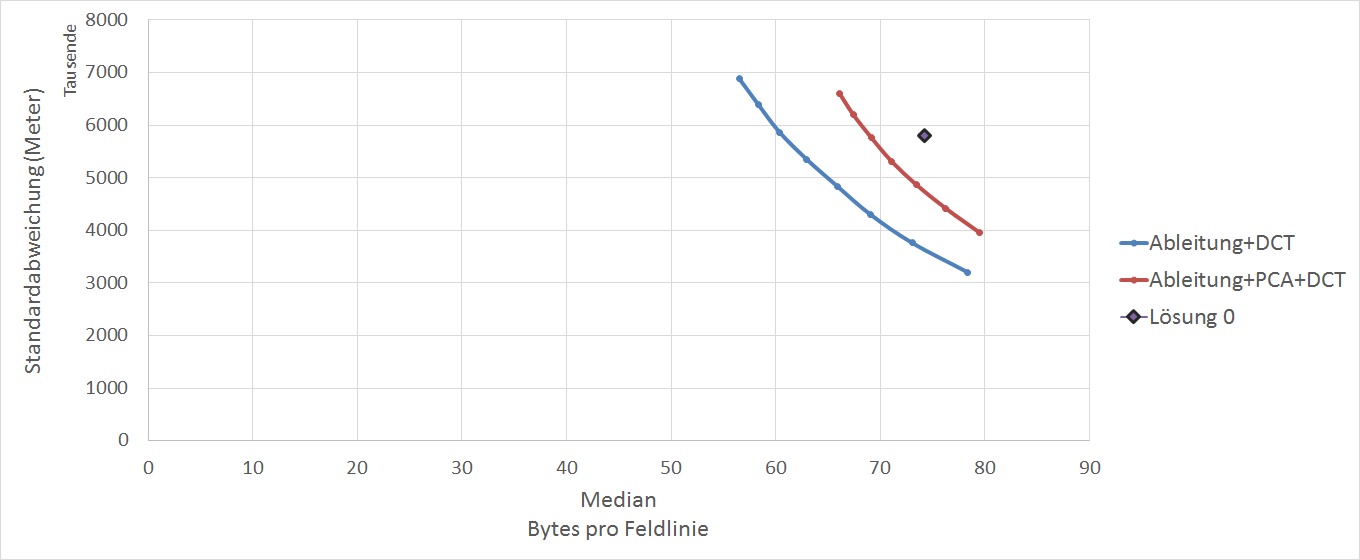
\includegraphics[width=0.8\textwidth,height=6cm,keepaspectratio]{./pictures/resultate/loesung1/loesung1-4/loesung1_4.png}
	\caption{Artefakte der DCT Kompression der Ableitung}
	\label{resultate:loesung1:dct:byte:artefakte:}
\end{figure} 
Die Abweichung ist in der selben Grössenordnung wie die der Lösung 0 \ref{resultate:loesung0:artefakte}. Von blossem Auge sind diese Artefakte nicht zu erkennen. Die Form er Linie wird erhalten. Ränder sind auch gut. jedoch scheint die pure DCT die Kurve besser approximieren zu können, falls die Ränder nicht wären.

\subsubsection{DCT mit Byte-Codierung}
Zum Vergleich wird das jetzt noch gemacht.

